\documentclass[Journal,letterpaper]{ascelike-new}
\usepackage{amsmath,amssymb}
\usepackage{booktabs}
\usepackage{graphicx}
\usepackage{multirow}
\usepackage[figurename=Fig.,labelfont=bf,labelsep=period]{caption}
% natbib removed for probe
\usepackage{url}
\usepackage[colorlinks=true,citecolor=red,linkcolor=black]{hyperref}

\newcommand{\fcntm}{FC-NTM}

\NameTag{Wang, \today}

\begin{document}

\title{Field-Cooperative Neural Topic Modeling of Civil Engineering Literature:
Read-out Evaluation and Missing-Abstract Inference}

\author[1]{Hongli Wang}
\author[1]{Qingpeng Man}

\affil[1]{School of Civil Engineering, Harbin Institute of Technology, Harbin, China.
E-mails: 2010254508@qq.com (H.~Wang); manqp@126.com (Q.~Man, corresponding author)}

\maketitle

\begin{abstract}
Title--abstract records are a core form of civil engineering literature, and part of most
collections is available with titles only. This paper studies how the two fields of such a record
should be modelled together, and what can still be inferred when the abstract is missing. We
present FC-NTM, a field-cooperative neural topic model with one conditional variational stream per
field, cross-field reconstruction, a consistency term and field-level masking, evaluated on civil
engineering records from OpenAlex together with two public short-text corpora. Under a unified
read-out protocol the civil corpus shows the largest and most consistent advantage: across ten
random seeds the class TF-IDF coherence is 0.049 and the native beta read-out 0.061 above BTM,
with ten positive pairs. A title-only routing task reaches 0.66 accuracy on fifteen external
automatic topic labels covering 42.9\% of the test records; the task is a routing aid and remains
below a supervised TF-IDF classifier. Cross-domain evaluations and read-out protocols are
reported in the paper and supplement, and per-seed results, fixed data splits and
hyper-parameters are released with the code.
\end{abstract}

\KeyWords{topic model; field cooperation; neural variational inference; fielded documents with short summary fields; class TF--IDF read-out; complementarity measures}

\section{Introduction}

Topic models summarise unlabelled collections as readable topic structures and are widely used in
news, software repositories and social media analysis. In many of these collections a record is not
a homogeneous bag of words but a pair of fields with different functions: a title that gives a
highly compressed summary, and a body that supplies context, motivation and qualifications. The
same topic is expressed differently in the two fields -- the body side tends to carry context and
causes, the summary side tends to carry objects and actions. Civil and construction engineering
records are a natural instance: bibliographic title--abstract pairs, technical specifications and
contract clauses, and accident reports all pair a short summary-like field with a longer contextual
field. Topic modelling of such documents is useful both for literature navigation and for records
whose long field is unavailable, for example when only titles have been collected.

Topic modelling has moved from probabilistic graphical models to neural variational models. LDA is
the classical bag-of-words Bayesian model \cite{blei2003lda}; GSDMM addresses short texts with a
collapsed Gibbs Dirichlet--multinomial mixture \cite{yin2014gsdmm}; AVITM introduces a linear
decoder into a variational auto-encoder and defines the LDA and ProdLDA generative processes
\cite{srivastava2017avitm}; NVDM applies variational auto-encoders to text early on
\cite{miao2016nvdm}; CTM/CombinedTM combine contextual sentence embeddings with bag-of-words
counts \cite{bianchi2021ctm}; ETM defines topics in a word-embedding space \cite{dieng2020etm};
BTM models word pairs instead of document-level counts and remains a strong baseline for short
texts \cite{yan2013btm}. Surveys note that structured and short-text corpora are still open
problems for neural topic models \cite{wu2024survey}.

Existing neural topic models exploit the internal field structure of a document only to a limited
degree: the fields are usually concatenated into one bag of words and their division is discarded.
Multi-view and multi-source topic modelling has been explored for parallel corpora, multiple data
sources and cross-modal settings
\cite{kurle2019multisource,zhang2017robust,pergola2021disentangled,liu2022dualview}; structured
neural topic models for reviews encode user--item context and assign words to sentence-level
aspects \cite{esmaeili2019structured}; structural topic models describe metadata with
document-level covariates \cite{roberts2019stm}. Short-text work such as DV-BTM optimises two
views jointly \cite{liu2022dualview}, CRNTM reinforces topic
inference with context \cite{crntm2020}, and DVI-DTM learns dual-view representations for
interpretable dynamic topics \cite{dvidtm2026}. In these works the two views play known roles
(query--document, user--item, or aspect layers); the setting studied here differs: the two fields
of the \emph{same} record are modelled by separate variational streams, and their relation is
fixed by the record schema rather than inferred as an explicit latent variable.  Separate
encoders, posterior alignment and missing-view inference are building blocks adopted from this
literature; the contribution claimed here is the field-cooperative configuration and its
read-out protocol, not those building blocks themselves.

In engineering informatics, text mining has become a recognised analysis tool: content analysis and
classification of safety reports \cite{civilsafety2015,civilaccident2018}, automated classification
of regulations and contracts and extraction of contractual risk clauses
\cite{compliance2013,ontology2015,contract2022,risknlp2023}, and surveys of natural language processing for
construction \cite{civilnlp2021,civilnlp2023}. Topic models have entered the field as well: DUET
applies LDA topic modelling to social-media text for detecting physical events in urban areas
\cite{duet2019}, neural topic modelling has
been used to map machine-learning applications in buildings \cite{civiltopic2024}, and semantic
topic modelling has been used to build taxonomies for digital building passports \cite{passport2026}. In contrast to
these works, we do not treat the topic model as a feature extractor for a downstream classifier.
We study the \emph{internal} field structure of an engineering record: topic inference when a field
is missing, field-restricted read-out, and whether these read-outs can be measured reliably.

This paper makes two contributions. \textbf{Methodologically}, it proposes the field-cooperative
neural topic model \fcntm{}, which models the two fields of a record as two conditional variational
streams that share one linear topic decoder, adds cross-field reconstruction and a field
consistency regulariser, and handles partial and complete field absence with field-level word
masking and whole-field dropout; a single trained model yields both a decoder $\beta$ read-out and
a class TF--IDF read-out under a unified evaluation vocabulary. \textbf{Empirically}, the paper
does not claim that the mechanism beats classical baselines on arbitrary dual-field corpora.
It asks what field structure provides and whether the resulting gains can be measured reliably.
On the civil corpus and on GitHub issues (background/summary length ratio 12.9) and AG News (3.9)
we extend \fcntm{} and BTM to ten seeds: both read-outs favour \fcntm{} on the civil corpus
($+0.049$ class TF--IDF and $+0.061$ $\beta$ $C_V$, 10/10 seeds), the class TF--IDF read-out is
$+0.028$ $C_V$ above BTM on GitHub (95\% CI $[+0.012,+0.043]$, 9/10 seeds) and $-0.009$ on AG News
(CI includes zero, 3/10), while on the two public corpora the $\beta$ read-out is lower than BTM.
We therefore claim the multi-seed-supported read-out advantages on the civil corpus and on GitHub,
and report the absence of an advantage on AG News. Two field-relation measures
are tested as candidate predictors -- a held-out mutual-prediction score and a post-training
occlusion diagnostic -- and neither serves as a monotone criterion. The value of field cooperation
is thus restricted to reproducible field-restricted read-outs and to the behaviour of inference
under missing fields, not to an unconditional performance advantage.

\section{Related Work}

\subsection{Neural topic models}

Neural topic models are mostly built on variational auto-encoders: an encoder maps the document
bag of words to the parameters of a latent Gaussian posterior and a decoder generates word
distributions. NVDM applied variational auto-encoders to text \cite{miao2016nvdm}, ProdLDA
introduced a linear decoder with a readable topic--word matrix \cite{srivastava2017avitm},
CTM/CombinedTM concatenate pretrained sentence embeddings with bag-of-words counts
\cite{bianchi2021ctm}, and ETM defines topics in a continuous embedding space \cite{dieng2020etm}.
For short texts, BTM models word pairs rather than document-level counts \cite{yan2013btm}, while
BERTopic and Top2Vec build topic representations from class TF--IDF statistics and joint embeddings
respectively \cite{grootendorst2022bertopic,angelov2020top2vec}. Neural and regularised variants of
BTM include GraphBTM \cite{zhu2018graphbtm} and BCK-TM, which encodes word-pair correlation
knowledge into the prior \cite{zhang2020bcktm}; BigARTM provides a general additive regularisation
framework for multimodal topic modelling \cite{vorontsov2015bigartm}. Our decoder follows the linear
ProdLDA structure and adds topic orthogonality, dropout \cite{srivastava2014dropout} and
validation-based early stopping \cite{prechelt1998early}; short-text-specific decoders use topic
quantisation and negative sampling to sharpen assignments \cite{quantization2020}. We keep this
regularisation consistent across the neural baselines we implement ourselves, while the official
CombinedTM keeps its own training loop; learning rates and KL weights differ between models, so the
training objectives should not be described as identical.

\subsection{Multi-view and structured-document topic models}

Multi-view topic models share information between views of the same data: bilingual and
cross-lingual models, multi-source models and disentangled representation models
\cite{kurle2019multisource,zhang2017robust,pergola2021disentangled,liu2022dualview}. Structured
neural topic models for reviews encode user--item context and sentence-level aspect assignments
\cite{esmaeili2019structured}, neural models can also condition on metadata
\cite{card2018metadata}, and the structural topic model conditions topics on document metadata
\cite{roberts2019stm}.
Short-text-oriented dual-view work is closest to ours: DV-BTM learns two views jointly
\cite{liu2022dualview}, CRNTM strengthens inference with context \cite{crntm2020}, and DVI-DTM
combines a time-aware term view with a sentence view and adds interpretable topic descriptions
\cite{dvidtm2026}; related word-pair models address relations and sparsity
\cite{relationalbtm2018,sparsebtm2021}. Two further lines overlap partially. Multi-source
variational inference with per-source encoders, a shared latent code and divergence terms between
posteriors \cite{kurle2019multisource} and JMVAE, which aligns modality posteriors and can infer
a missing modality from the remaining one \cite{suzuki2017jmvae}, already contain separate
encoders, posterior alignment and missing-view inference; SubNTM instead models a hierarchy of
document and sub-document topics \cite{nguyen2026subntm}, i.e.\ structure \emph{inside} a field.
The setting studied here is defined by the record schema rather than by unknown view roles: two
textual fields of the same record share one bag-of-words vocabulary and one linear decoder, the
fields enter with fixed weights, and the evaluation asks what the field-restricted read-outs and
missing-background inference measure. Separate encoding, posterior alignment and missing-view
handling are therefore building blocks adopted from this literature rather than contributions
claimed as new here.

\subsection{Text mining and topic modelling of engineering documents}

Engineering informatics has accumulated a substantial body of text-mining work: content analysis
and classification of construction safety reports \cite{civilsafety2015,civilaccident2018},
automated classification of regulatory and contractual documents and extraction of risk clauses
\cite{compliance2013,ontology2015,contract2022,risknlp2023}, and domain surveys of natural language processing
for construction \cite{civilnlp2021,civilnlp2023}. Topic models have also been applied: DUET uses
LDA topic modelling on social-media text to detect physical events in urban areas \cite{duet2019},
recent work applies neural
topic modelling to map machine-learning applications in buildings \cite{civiltopic2024}, and
semantic topic modelling supports taxonomy construction for digital building passports \cite{passport2026}. These
studies use topics as inputs to downstream classification or as a mapping tool. We instead study
the field structure inside a single engineering record -- title versus abstract -- and ask when
field-restricted topics and missing-field inference are informative, and when the corresponding
gains are measurable.

\section{Method}

\subsection{Problem setting}

Each record $d$ consists of field A (\emph{background}, e.g.\ the abstract of a paper or the body
of an issue) and field B (\emph{summary}, e.g.\ the title), with $N$ records in total and a shared
evaluation vocabulary of $V$ terms. The model maintains $K$ topics, a document--topic distribution
$\theta_d\in\Delta^{K-1}$, and a topic--word matrix $\beta\in\mathbb{R}^{K\times V}$ shared by both
fields. The task is to infer $\theta_d$ and $\beta$ from unlabelled records, to produce readable
topics in two read-outs, and to remain usable when one field is partially or entirely missing at
inference time.

\subsection{Field streams and the shared decoder}

Each field is encoded by its own two-layer MLP encoder (200 hidden units, Softplus activations,
dropout $0.2$) into the parameters of a field-conditioned Gaussian posterior,
\begin{equation}
q_f(z_f\mid x_f)=\mathcal N\big(\mu_f(x_f),\operatorname{diag}(\sigma_f^2(x_f))\big),
\qquad f\in\{\mathrm{bg},\mathrm{sm}\},
\end{equation}
where $x_f$ is the $L_1$-normalised bag of words of field $f$ and $\log\sigma_f^2$ is capped at
$2$. Posterior means are mapped to topic proportions by a deterministic softmax,
$\bar\theta_f=\operatorname{softmax}(\mu_f(x_f))$, which is used at evaluation time in place of
sampling; $\bar\theta_f$ is therefore a deterministic topic-proportion estimate, not the
expectation of $\operatorname{softmax}(z_f)$. Both streams share one linear topic--word matrix
$W\in\mathbb{R}^{K\times V}$, and write $\theta_f\in\mathbb{R}^{1\times K}$ for the topic
proportions of field $f$ under the row-vector convention,
\begin{equation}
p(w\mid\theta_f)=\operatorname{softmax}\!\big(\mathrm{BN}(\theta_f W)\big),
\label{eq:decode}
\end{equation}
where $\theta_f$ passes through dropout before the product, $\mathrm{BN}$ is a batch-normalisation
layer \emph{without} affine parameters applied over the vocabulary dimension (batch statistics
during training, running statistics at evaluation), and there is no additive bias. The $\beta$
read-out of the ``Unified topic-word read-out'' subsection reads the raw rows of $W$, whereas generation uses the
normalised path of Eq.~\eqref{eq:decode}; the gap between the two is quantified in the
Supplementary Material.

\subsection{Training objective}

For a document $d$ let $\mathcal{G}_d$ collect its present fields (the background field is present
when the record carries it; the summary stream is always instantiated, including zero-vector
inputs after preprocessing) and let
$\mathcal{A}_d\subseteq\mathcal{G}_d$ be the \emph{active streams}, i.e.\ present fields whose
stream is not removed by whole-field dropout. Write $n^{(g)}_{dw}$ for the raw count of word $w$
in field $g$. Each active stream decodes once (Eq.~\eqref{eq:decode}) and reconstructs
\emph{every present field},
\begin{equation}
R_f=\sum_{g\in\mathcal{G}_d}\omega_g\,R_f(g),\qquad
R_f(g)=-\sum_{w=1}^{V} n^{(g)}_{dw}\,\log p\!\left(w\mid\theta_f\right),
\label{eq:recon}
\end{equation}
with fixed field weights $\omega_{\mathrm{bg}}=2.0$ and $\omega_{\mathrm{sm}}=1.0$. The summary
stream therefore reconstructs the background field as well (cross-field reconstruction), and a
background field that was observed but dropped during training stays in the reconstruction
targets even though its own stream is inactive, whereas a naturally missing background field
enters neither the inputs nor the targets. The per-document objective is
\begin{equation}
\mathcal{L}_d=\frac{1}{|\mathcal{A}_d|}\sum_{f\in\mathcal{A}_d}
\Big[R_f+\lambda_{\mathrm{KL}}(t)\,\mathrm{KL}_f\Big]
+\lambda_f R_{\mathrm{fuse}}+\lambda_{\mathrm{JS}}\,\mathrm{JS},
\label{eq:total}
\end{equation}
where $\mathrm{KL}_f=\mathrm{KL}\big(q_f(z_f\mid x_f)\,\|\,\mathcal N(0,I)\big)$ is summed over
the $K$ latent dimensions and clamped at zero, and $\lambda_{\mathrm{KL}}(t)=0.05\min(1,t/20)$
anneals linearly during the first 20 epochs. The fused term
$R_{\mathrm{fuse}}=\sum_{g\in\mathcal{G}_d}\omega_g R_{\mathrm{fuse}}(g)$ is a second
reconstruction of both present fields from the fused topic mixture
\begin{equation}
\theta_d^{\mathrm{fuse}}=g\,\theta_{\mathrm{bg}}+(1-g)\,\theta_{\mathrm{sm}},
\qquad g=\sigma(w),\quad w\in\mathbb{R},
\label{eq:lfuse}
\end{equation}
for records with both fields present, and
$\theta_d^{\mathrm{fuse}}=\theta_{\mathrm{sm}}$ when the background field is missing or
dropped. During training Eq.~\eqref{eq:lfuse} combines the \emph{sampled} per-stream
proportions that also feed the per-stream reconstructions; at inference time, and for the JS
term below, the deterministic estimates $\bar\theta_f$ are used instead, so at inference
Eq.~\eqref{eq:lfuse} is a convex combination of two deterministic topic-proportion estimates,
which is why we call it a \emph{fused topic mixture} rather than a posterior. The gate
$g$ receives gradients only through $R_{\mathrm{fuse}}$, so with $\lambda_f=0$ the model
degenerates exactly to fixed mean fusion. The consistency term
\begin{equation}
\mathrm{JS}=\tfrac12\,\mathrm{KL}\!\big(\bar\theta_{\mathrm{bg}}\|m\big)
+\tfrac12\,\mathrm{KL}\!\big(\bar\theta_{\mathrm{sm}}\|m\big),
\qquad m=\tfrac12\big(\bar\theta_{\mathrm{bg}}+\bar\theta_{\mathrm{sm}}\big),
\end{equation}
acts on the deterministic topic proportions, not on the Gaussian posteriors, and is computed only
for documents whose two streams are both active, so no record is implicitly regularised more
strongly than another. A topic-orthogonality penalty keeps the rows of $W$ apart,
\begin{equation}
\Omega=\frac{1}{K(K-1)}\sum_{k\neq k'}\big|\cos\langle W_k,W_{k'}\rangle\big|,
\end{equation}
and the batch objective is $\frac{1}{|B|}\sum_{d\in B}\mathcal{L}_d
+\lambda_{\mathrm{orth}}\Omega$ with $\lambda_{\mathrm{orth}}=0.2$.

Two masking mechanisms expose the model to missing fields, and they act on different units.
(i) \emph{Word-level input dropout} (denoising) is applied during training to the bag-of-words
\emph{word types} of each field: each BoW dimension is independently zeroed with probability
$0.30$ (background) or $0.40$ (summary) in the encoder view only, while the reconstruction
targets remain the complete counts. (ii) \emph{Whole-field dropout} removes the background stream
of each training document with probability $0.5$ and substitutes the prior; the summary stream is
never dropped and learns to reconstruct both fields on its own. The test-time occlusion protocol
of the ``Field inference under partial occlusion'' subsection instead masks \emph{token positions} in the raw field text, so the
training and evaluation units should not be conflated. The consistency weight
$\lambda_{\mathrm{JS}}=0.5$, the fusion weight $\lambda_f=0.5$ and the dropout probabilities were
selected on held-out data.

\subsection{Optimisation}

Training uses Adam (learning rate $5\times10^{-4}$, momentum parameters $0.9$ and $0.999$),
mini-batches of $128$, gradient-norm clipping at $5.0$ and a budget of $700$ epochs. After the KL
warm-up the state with the lowest held-out loss is kept, for which $20\%$ of the training split is
held out; the patience is $150$ epochs. Evaluation-mode inference is deterministic: the
reparameterisation sampling is switched off and the held-out loss uses posterior means.
Numerical-anomaly recovery rolls the weights back to the most recent finite epoch, clears the
optimiser moments and halves the learning rate; this recovery step is separate from the
best-held-out-epoch selection of the early-stopping loop.

\subsection{Unified topic-word read-out}
\label{sec:readout}

Topic-word comparisons are only meaningful if every model is read out with the same vocabulary and
the same number of words per topic. We therefore fix one evaluation vocabulary and exactly ten
words per topic. The \textbf{$\beta$ read-out} takes the top ten words of each normalised row of
the model's topic--word matrix; for \fcntm{} these are the raw rows of $W$, whereas generation
uses Eq.~\eqref{eq:decode}. LDA, BTM, NMF, ProdLDA, ETM, CTM-lite, CombinedTM and \fcntm{} are all
evaluated this way. The \textbf{class TF--IDF read-out} aggregates the training-term counts by the
soft document--topic assignment of the model, applies a BERTopic-style class TF--IDF transform,
and then takes the top ten words; for \fcntm{} this read-out is built from the fused topic mixture
$\bar\theta^{\mathrm{fuse}}$, which is why the two read-outs can rank models differently. The
sensitivity of the raw-parameter read-out relative to the generative read-out is reported in the
Supplementary Material.

\section{Experiments}

\subsection{Corpora and evaluation protocol}

We use three dual-field corpora. The \textbf{civil engineering corpus} is the application corpus:
title--abstract records of English journal articles from OpenAlex \cite{openalex2022} in \emph{Civil and Structural
Engineering} and \emph{Building and Construction} (2000--2023, CC-licensed records only), 6000
training and 2000 test records, with the title as the summary field and the abstract as the
background field (mean length ratio 11.2). \textbf{GitHub issues} \cite{openindex2026} pairs the
issue body with its title (four mature repositories, 6000/2000, ratio 12.9), and \textbf{AG News}
\cite{zhang2015char} pairs the description
with the headline (6000/7600, ratio 3.9). All corpora are lower-cased and tokenised on letter
sequences; stop words and very short tokens are removed, the vocabulary is built from the training
split only, and test records never enter the vocabulary. Table~\ref{tab:civil} reports the
application corpus and Tables~\ref{tab:agnews} and~\ref{tab:github} the two public corpora, all on
the same evaluation vocabulary with exactly ten words per topic and $K=30$. The evaluation
protocol (vocabulary, ten words per topic, coherence and
diversity metrics) is shared by every model, whereas the training procedure differs across
algorithm families and is described in the ``Baselines, training protocols and metrics'' subsection. Because a 400-record
development subset was used during design, every result is also
recomputed on a development-free test subset (1600 GitHub and 7200 AG News records); the
re-scoring removes direct test overlap only and cannot undo the model selection that already
happened, so it is reported as a sensitivity analysis rather than as an untouched confirmation
set. The results are organised around three questions: how well civil title--abstract records can
be structured into verifiable topics; how much signal remains when the abstract is missing; and
how much the complete field-cooperative configuration adds over a concatenated single-encoder
control. Cross-corpus diagnostics support these questions rather than replacing them.

\subsection{Baselines, training protocols and metrics}
\label{sec:protocol}

Baselines are LDA \cite{blei2003lda}, BTM \cite{yan2013btm}, NMF with a KL objective
\cite{lee2001nmf}, ProdLDA \cite{srivastava2017avitm}, ETM \cite{dieng2020etm}, CTM-lite, the
official CombinedTM \cite{bianchi2021ctm}, BERTopic \cite{grootendorst2022bertopic} and Top2Vec
\cite{angelov2020top2vec}; contextual baselines use Sentence-BERT embeddings
\cite{reimers2019sbert}. The implementations fall into four families whose training procedures
differ, and they are not interchangeable training loops. (i) \emph{Gibbs sampling}: BTM is a
collapsed Gibbs sampler over biterms (word pairs within a window of 12 tokens, at most 150 sampled
pairs per document, $\alpha=50/K$, $\beta=0.01$, 300 full sweeps); LDA is fitted by gensim's batch
variational Bayes (50 passes, 120 iterations per pass, symmetric $\alpha$). (ii) \emph{Matrix
factorisation}: NMF minimises the Kullback--Leibler divergence between the count matrix and $WH$
with multiplicative updates (600 iterations, tolerance $10^{-4}$). (iii) \emph{Neural variational
models}: ProdLDA, ETM, CTM-lite and \fcntm{} share the same Adam loop, mini-batch size and budget
(700 epochs, 20\% held-out early stopping), but the learning rate differs -- the baselines use
$2\times10^{-3}$, the main \fcntm{} configuration uses $5\times10^{-4}$ selected on development
data -- and the official CombinedTM keeps its own training loop (Adam, learning rate
$2\times10^{-3}$, batch size $64$, 700 epochs, early stopping on its own held-out split).
(iv) \emph{Embedding-clustering models} choose their own topic numbers: BERTopic runs UMAP
followed by HDBSCAN with fixed random seeds, and Top2Vec fits Doc2Vec document vectors followed by
HDBSCAN; both are reported for reference only. Quality is measured by $C_V$ coherence
\cite{roder2015coherence}, NPMI
\cite{bouma2009npmi,lau2014tea}, UCI and UMass, IRBO topic diversity \cite{webber2010rbo} and a
$K$-corrected exclusivity $EXCL_{KADJ}$ \cite{bischof2012exclusivity}; coherence scores drop
topics with non-finite scores, so we record the effective topic count next to every score.
Definitions of the two corrected measures are given in the Supplementary Material.

 \begin{table}[t]
\centering
\caption{Topic quality on the civil engineering corpus (unified evaluation vocabulary, ten words per topic; values are means over seeds 11/23/37, and the training procedure differs across algorithm families as described in the ``Baselines, training protocols and metrics'' subsection; BERTopic and Top2Vec choose their own topic numbers and are shown for reference).}
\label{tab:civil}
\small
\begin{tabular}{lcccccc}
\toprule
Model & Topics & $C_V$ & NPMI & UMass & EXCL$_{\mathrm{KADJ}}$ & IRBO \\
\midrule
BTM & 30 & 0.583$\pm$0.010 & 0.128$\pm$0.009 & $-$2.18 & 0.283 & 0.944 \\
CombinedTM & 30 & 0.539$\pm$0.029 & 0.082$\pm$0.028 & $-$6.11 & 0.063 & 0.998 \\
\fcntm{}-cTFIDF & 30 & \textbf{0.636}$\pm$0.014 & \textbf{0.159}$\pm$0.011 & $-$2.21 & 0.165 & 0.937 \\
\fcntm{} & 30 & 0.633$\pm$0.014 & 0.154$\pm$0.022 & $-$2.85 & 0.014 & 0.990 \\
ETM & 30 & 0.581$\pm$0.012 & 0.119$\pm$0.007 & $-$2.75 & 0.379 & 0.963 \\
ProdLDA & 30 & 0.580$\pm$0.023 & 0.125$\pm$0.017 & $-$3.84 & 0.051 & 0.999 \\
Top2Vec & 153 & 0.515$\pm$0.002 & 0.029$\pm$0.011 & $-$8.52 & 0.359 & 0.995 \\
NMF & 30 & 0.598$\pm$0.009 & 0.135$\pm$0.006 & $-$2.86 & 0.559 & 0.984 \\
BERTopic & 29 & 0.576$\pm$0.026 & 0.116$\pm$0.027 & $-$5.06 & 0.563 & 0.991 \\
CTM-lite & 30 & 0.536$\pm$0.030 & 0.098$\pm$0.027 & $-$3.85 & 0.013 & 0.995 \\
LDA & 30 & 0.554$\pm$0.008 & 0.056$\pm$0.025 & $-$4.62 & 0.602 & 0.987 \\
\bottomrule
\end{tabular}
\end{table}

\begin{table}[t]
\centering
\caption{Topic quality on AG News (unified evaluation vocabulary, ten words per topic; values are means over seeds 11/23/37 where applicable, and the training procedure differs across algorithm families as described in the ``Baselines, training protocols and metrics'' subsection; BERTopic and Top2Vec choose their own topic numbers and are shown for reference).}
\label{tab:agnews}
\small
\begin{tabular}{lcccccc}
\toprule
Model & Topics & $C_V$ & NPMI & UMass & EXCL$_{\mathrm{KADJ}}$ & IRBO \\
\midrule
BTM & 30 & 0.600$\pm$0.011 & 0.164$\pm$0.005 & $-$4.19 & 0.409 & 0.980 \\
CombinedTM & 30 & 0.526$\pm$0.037 & 0.057$\pm$0.070 & $-$8.01 & 0.118 & 1.000 \\
\fcntm{}-cTFIDF & 30 & \textbf{0.612}$\pm$0.014 & \textbf{0.173}$\pm$0.012 & $-$4.20 & 0.193 & 0.974 \\
\fcntm{} & 30 & 0.586$\pm$0.026 & 0.137$\pm$0.022 & $-$4.91 & 0.013 & 0.993 \\
ETM & 30 & 0.506$\pm$0.014 & 0.092$\pm$0.010 & $-$5.12 & 0.439 & 0.982 \\
ProdLDA & 30 & 0.526$\pm$0.031 & 0.071$\pm$0.015 & $-$6.61 & 0.055 & 0.999 \\
Top2Vec & 2.7 & 0.498$\pm$0.032 & 0.099$\pm$0.031 & $-$2.92 & 0.268 & 0.937 \\
NMF & 30 & 0.494$\pm$0.015 & 0.069$\pm$0.013 & $-$5.96 & 0.799 & 0.997 \\
BERTopic & 29 & 0.488$\pm$0.022 & 0.035$\pm$0.026 & $-$8.81 & 0.681 & 0.997 \\
CTM-lite & 30 & 0.431$\pm$0.023 & $-$0.015$\pm$0.016 & $-$8.34 & 0.041 & 0.998 \\
LDA & 30 & 0.421$\pm$0.013 & $-$0.066$\pm$0.018 & $-$8.62 & 0.696 & 0.994 \\
\bottomrule
\end{tabular}
\end{table}

\begin{table}[t]
\centering
\caption{Topic quality on GitHub issues (same evaluation protocol and read-outs as Table~\ref{tab:agnews}; the FC-NTM rows, BTM, ETM, CombinedTM, ProdLDA and CTM-lite are three-seed results).}
\label{tab:github}
\small
\begin{tabular}{lcccccc}
\toprule
Model & Topics & $C_V$ & NPMI & UMass & EXCL$_{\mathrm{KADJ}}$ & IRBO \\
\midrule
BTM & 30 & 0.712$\pm$0.012 & 0.232$\pm$0.012 & $-$1.79 & 0.349 & 0.934 \\
\fcntm{}-cTFIDF & 30 & \textbf{0.727}$\pm$0.022 & \textbf{0.274}$\pm$0.026 & $-$1.90 & 0.133 & 0.901 \\
\fcntm{} & 30 & 0.701$\pm$0.016 & 0.233$\pm$0.012 & $-$3.16 & 0.010 & 0.967 \\
ETM & 30 & 0.675$\pm$0.014 & 0.213$\pm$0.010 & $-$2.14 & 0.366 & 0.955 \\
CombinedTM & 30 & 0.643$\pm$0.022 & 0.193$\pm$0.015 & $-$4.70 & 0.031 & 0.983 \\
NMF & 30 & 0.614$\pm$0.005 & 0.164$\pm$0.003 & $-$3.26 & 0.595 & 0.985 \\
ProdLDA & 30 & 0.579$\pm$0.007 & 0.107$\pm$0.012 & $-$5.21 & 0.043 & 0.995 \\
CTM-lite & 30 & 0.585$\pm$0.032 & 0.129$\pm$0.036 & $-$5.11 & 0.011 & 0.989 \\
LDA & 30 & 0.546$\pm$0.011 & 0.074$\pm$0.017 & $-$4.21 & 0.684 & 0.990 \\
BERTopic & 29 & 0.540$\pm$0.015 & 0.076$\pm$0.012 & $-$7.00 & 0.546 & 0.976 \\
Top2Vec & 160 & 0.493$\pm$0.009 & $-$0.008$\pm$0.013 & $-$9.65 & 0.337 & 0.994 \\
\bottomrule
\end{tabular}
\end{table}

\subsection{Main results}

On the civil engineering corpus (Table~\ref{tab:civil}), \fcntm{} attains the highest coherence
among all evaluated models under both read-outs ($C_V=0.633$ for the $\beta$ read-out and $0.636$ for
the class TF--IDF read-out; NPMI $0.154$ and $0.159$ over seeds 11/23/37), ahead of NMF (0.598),
BTM (0.583) and the neural baselines, and the ten-seed extension keeps both read-out advantages
(Table~\ref{tab:seed-paired}).
On AG News, \fcntm{}-cTFIDF reaches $C_V=0.612$ and NPMI $=0.173$, above BTM under the matched
class TF--IDF read-out ($0.593$ / $0.169$) and clearly above the $\beta$ read-outs of ProdLDA,
ETM, NMF, CTM-lite and LDA; under its own $\beta$ read-out BTM keeps a small lead ($0.600$ versus $0.586$). On GitHub issues, \fcntm{}-cTFIDF reaches $C_V=0.727$ and NPMI $=0.274$,
above BTM at both read-outs ($0.712$ / $0.232$ for the native $\beta$ read-out, $0.700$ / $0.235$
matched), and above the sentence-embedding baselines (CombinedTM $0.643$, BERTopic $0.540$).
The matched-read-out advantage over BTM is therefore $+0.027$ $C_V$ and $+0.039$ NPMI on GitHub and
$+0.019$ / $+0.004$ on AG News for three seeds, but the per-seed structure differs: on GitHub all
three seeds are positive, whereas the AG News mean is carried by two of three seeds and the NPMI
advantage by one. On the development-free test subset the ordering is unchanged
(GitHub $0.734$ versus $0.711$, NPMI $0.284$ versus $0.248$; AG News $0.610$ versus $0.590$, NPMI
$0.172$ versus $0.167$; with BTM's native $\beta$ read-out, $0.734$ versus $0.726$ and $0.610$
versus $0.598$).

\begin{figure}[t]
\centering
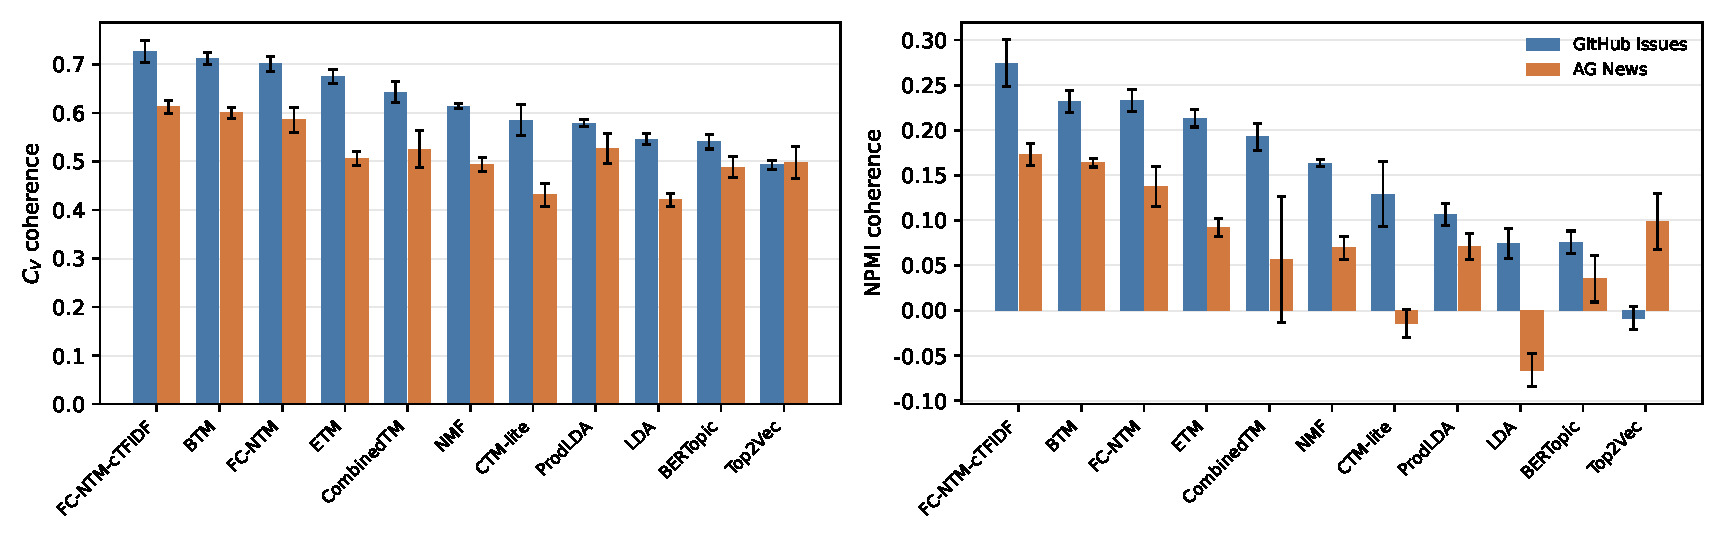
\includegraphics[width=0.86\textwidth]{fig_main_comparison_en.pdf}
\caption{Main results on the two public corpora (unified evaluation vocabulary, ten words per
topic). Left: $C_V$; right: NPMI. Error bars are standard deviations across seeds. The \fcntm{}
rows, BTM and ETM on GitHub and the \fcntm{} rows on AG News are three-seed results; CombinedTM,
ProdLDA and CTM-lite were run for the same seeds 11/23/37 under the same protocol.}
\label{fig:main}
\end{figure}

\subsection{Read-out-matched comparison}

\begin{table}[t]
\centering
\caption{Read-out comparison ($K=30$, means over seeds 11/23/37). Each model is first read out through its own topic--word matrix ($\beta$ read-out) and then through a class TF--IDF read-out aggregated from its training-set posterior $\theta$; BTM enters the same read-out through the point-estimate document--topic posterior of its original Section 3.3, and the FC-NTM row is the same model as in Tables~\ref{tab:agnews} and~\ref{tab:github}.}
\label{tab:fair}
\footnotesize
\setlength{\tabcolsep}{4pt}
\begin{tabular}{@{}llcc@{}}
\toprule
Corpus & Model & $\beta$ read-out $C_V$ / NPMI & Class TF--IDF $C_V$ / NPMI \\
\midrule
 \multirow{7}{*}{GitHub}
 & \fcntm{}(3 seed mean) & 0.701 / 0.233 & \textbf{0.727 / 0.274} \\
 & ETM & 0.675 / 0.213 & 0.669 / 0.220 \\
 & ProdLDA & 0.579 / 0.107 & 0.666 / 0.215 \\
 & CTM-lite & 0.585 / 0.129 & 0.675 / 0.216 \\
 & NMF & 0.614 / 0.164 & 0.603 / 0.158 \\
 & LDA & 0.546 / 0.074 & 0.614 / 0.193 \\
 & BTM(3 seeds) & 0.712 / 0.232 & 0.700 / 0.235 \\
\midrule
 \multirow{7}{*}{AG News}
 & \fcntm{}(3 seed mean) & 0.586 / 0.137 & \textbf{0.612 / 0.173} \\
 & ProdLDA & 0.526 / 0.071 & 0.544 / 0.125 \\
 & NMF & 0.494 / 0.069 & 0.539 / 0.121 \\
 & ETM & 0.506 / 0.092 & 0.511 / 0.082 \\
 & CTM-lite & 0.431 / $-$0.015 & 0.455 / 0.062 \\
 & LDA & 0.421 / $-$0.066 & 0.451 / 0.010 \\
 & BTM(3 seeds) & 0.600 / 0.164 & 0.593 / 0.169 \\
\midrule
 \multirow{7}{*}{Civil corpus}
 & \fcntm{}(3 seed mean) & \textbf{0.633 / 0.154} & \textbf{0.636 / 0.159} \\
 & NMF & 0.598 / 0.135 & 0.607 / 0.142 \\
 & ETM & 0.581 / 0.119 & 0.603 / 0.134 \\
 & BTM(3 seeds) & 0.583 / 0.128 & 0.590 / 0.139 \\
 & LDA & 0.554 / 0.056 & 0.575 / 0.105 \\
 & ProdLDA & 0.580 / 0.125 & 0.545 / 0.108 \\
 & CTM-lite & 0.536 / 0.098 & 0.530 / 0.094 \\
\bottomrule
\end{tabular}
\end{table}

The class TF--IDF read-out is strong but its effect depends on the model and the corpus: on GitHub
it lifts CTM-lite, ProdLDA and LDA by $0.091$, $0.087$ and $0.068$ but leaves ETM ($-0.006$) and
NMF ($-0.011$) unchanged or worse, while on AG News it helps every model except BTM by
$+0.005$--$+0.045$. Comparing \fcntm{}-cTFIDF against baselines read out with their own $\beta$
matrix therefore mixes the model and the read-out; every model-quality statement below therefore uses the matched comparison. Under the matched read-out the strongest baselines on GitHub are BTM ($0.700$),
CTM-lite ($0.675$), ETM ($0.669$) and ProdLDA ($0.666$), and \fcntm{}-cTFIDF leads them by
$0.027$--$0.061$ $C_V$ and $0.039$--$0.059$ NPMI, larger than its seed-to-seed standard deviation
($0.022$). On AG News the matched advantage is $+0.019$ $C_V$ over BTM but only two of three seeds
are positive and the NPMI advantage rests on one seed, while under the native $\beta$ read-out
\fcntm{} is below BTM ($0.586$ versus $0.600$). On the civil corpus the strongest
matched-read-out baselines are NMF ($0.607$) and ETM ($0.603$), ahead of BTM ($0.590$);
\fcntm{}-cTFIDF leads them by $0.029$ and $0.033$ $C_V$, but the ten-seed paired comparison is
against BTM, so the multi-seed civil evidence is specific to that comparison. The stable gains are therefore concentrated on the matched read-out, with a corpus-specific pattern. Two caveats apply: the class TF--IDF transform does not
automatically favour BTM (its $C_V$ drops from $0.712$ to $0.700$ on GitHub and from $0.600$ to
$0.593$ on AG News), so its direction must be measured rather than assumed; and the architecture
hyper-parameters of \fcntm{} were selected on development data while the baselines use their
defaults, a tuning-budget difference that the read-out comparison cannot remove.

\subsection{Ten-seed paired comparison}

To test whether the three-seed differences are seed noise, we extend \fcntm{} and BTM to ten seeds
on all three corpora (adding 53/71/89/101/113/127/139) and compare both read-outs and the
occlusion behaviour seed by seed; the occlusion rows use pre-selected baselines (BTM on all three
corpora and additionally LDA on AG News) rather than a full tournament.

\begin{table}[t]
\centering
\caption{Ten-seed paired comparison of \fcntm{} and BTM on the three corpora. The read-out rows report $C_V$ differences (\fcntm{} minus BTM at the same read-out); the occlusion rows compare the relative degradation $\mathrm{NLL}(100\%)/\mathrm{NLL}(25\%)$, so a positive value means \fcntm{} is more stable. The occlusion rows use the pre-selected baselines (BTM on all three corpora and additionally LDA on AG News) rather than a full baseline tournament. CIs are two-sided $t$ intervals; sign and Wilcoxon tests are two-sided.}
\label{tab:seed-paired}
\small
\setlength{\tabcolsep}{4pt}
\begin{tabular}{@{}llcccccc@{}}
\toprule
Corpus & Comparison & Mean diff. & 95\% CI low & 95\% CI high & Positive & Sign $p$ & Wilcoxon $p$ \\
\midrule
GitHub & Class TF--IDF & $+$0.028 & $+$0.012 & $+$0.043 & 9/10 & 0.021 & 0.004 \\
GitHub & $\beta$ read-out & $-$0.014 & $-$0.028 & $-$0.001 & 3/10 & 0.344 & 0.037 \\
GitHub & Occlusion (vs.\ BTM) & $+$0.024 & $+$0.022 & $+$0.026 & 10/10 & 0.002 & 0.002 \\
\midrule
AG News & Class TF--IDF & $-$0.009 & $-$0.030 & $+$0.013 & 3/10 & 0.344 & 0.375 \\
AG News & $\beta$ read-out & $-$0.027 & $-$0.047 & $-$0.008 & 1/10 & 0.021 & 0.004 \\
AG News & Occlusion (vs.\ BTM) & $+$0.025 & $+$0.024 & $+$0.026 & 10/10 & 0.002 & 0.002 \\
AG News & Occlusion (vs.\ LDA) & $-$0.013 & $-$0.014 & $-$0.012 & 0/10 & 0.002 & 0.002 \\
\midrule
Civil corpus & Class TF--IDF & $+$0.049 & $+$0.033 & $+$0.064 & 10/10 & 0.002 & 0.002 \\
Civil corpus & $\beta$ read-out & $+$0.061 & $+$0.047 & $+$0.075 & 10/10 & 0.002 & 0.002 \\
Civil corpus & Occlusion (vs.\ BTM) & $-$0.003 & $-$0.004 & $-$0.002 & 0/10 & 0.002 & 0.002 \\
\bottomrule
\end{tabular}
\end{table}

Four observations follow. First, the matched read-out advantage on GitHub survives ten seeds:
\fcntm{}-cTFIDF is $+0.028$ $C_V$ above BTM (95\% CI $[+0.012,+0.043]$, 9/10 seeds positive) and
its relative degradation advantage is $+0.024$ (10/10, $p=0.002$). Second, the civil corpus gives
the largest and most consistent read-out advantage: $+0.049$ class TF--IDF and $+0.061$ native
$\beta$ $C_V$ (the latter refers to the raw-parameter read-out; the BN-generated counterpart
is smaller, see the Supplementary Material), both with all ten paired differences positive
($p=0.002$), although the occlusion
ratio still favours BTM ($-0.003$, 0/10). Third, the three-seed AG News advantage is not replicated under ten seeds: the matched read-out difference is $-0.009$, with a confidence interval that includes zero (3/10). Fourth, on the
two public corpora the native $\beta$ read-out is below BTM ($-0.014$ and $-0.027$); overall the
advantage is corpus-dependent and read-out-dependent: largest on the civil corpus under both
read-outs, moderate and class-TF--IDF-focused on GitHub, and neutral on AG News. Confidence intervals
describe training (and masking) randomness under a fixed corpus and a fixed design; the $p$-values
are exploratory and not corrected for multiple comparisons.

\subsection{Field redundancy and the gain}

\begin{table}[t]
\centering
\caption{Field redundancy, measured occlusion gap and the $C_V$ difference against BTM on two corpora. Redundancy is fitted on the training split and evaluated on the test split and includes constructive controls (exact copy $=1.000$, cross-document shuffle $\approx0.000$); the occlusion $\Delta C_V$ is the mean$\pm$standard deviation over seeds 11/23/37 with dropout training. The last column gives the $C_V$ difference under the matched class TF--IDF read-out and under BTM's native $\beta$ read-out.}
\label{tab:conditional}
\footnotesize
\setlength{\tabcolsep}{4pt}
\begin{tabular}{@{}lcccc@{}}
\toprule
Corpus & Held-out Ridge $R^2$ & Held-out $\rho^2_{\mathrm{cca}}$
 & Occlusion $\Delta C_V$ & $C_V$ gap, cTFIDF$-$BTM (matched / $\beta$) \\
\midrule
GitHub issues & 0.230 & 0.306 & $+$0.009$\pm$0.022 & $+$0.027 / $+$0.014 \\
AG News & 0.158 & 0.245 & $+$0.018$\pm$0.013 & $+$0.019 / $+$0.012 \\
\bottomrule
\end{tabular}
\end{table}

\begin{figure}[t]
\centering
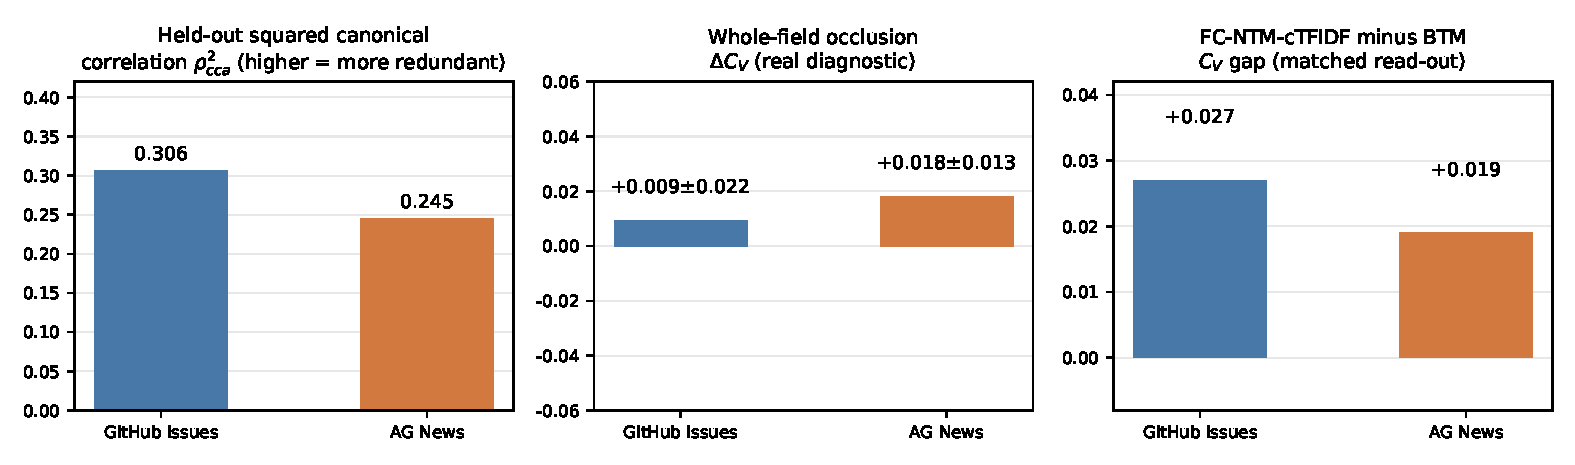
\includegraphics[width=0.86\textwidth]{fig_complementarity_en.pdf}
\caption{Field redundancy and gain (held-out measures). Left: squared canonical correlation $\rho^2_{\mathrm{cca}}$ (higher means more redundant; fitted on the training split and evaluated on the test split); middle: the $\Delta C_V$ of the real occlusion diagnostic (GitHub $+0.009\pm0.022$, AG News $+0.018\pm0.013$, three seeds each); right: the $C_V$ difference between \fcntm{}-cTFIDF and BTM under the matched read-out (GitHub $+0.027$, AG News $+0.019$). The two corpora have similar redundancy, while the ten-seed gain is positive on GitHub only (AG News $-0.009$), so the figure does not support a redundancy-based prediction of the gain.}\label{fig:cond}
\end{figure}

The redundancy measures are fitted on the training split and evaluated on the test split. The two
corpora have almost the same held-out predictability (GitHub is slightly higher,
$\rho^2_{\mathrm{cca}}$ 0.306 versus 0.245), while \fcntm{}-cTFIDF is slightly above BTM on both at
three seeds ($+0.027$ and $+0.019$ matched) and the ten-seed extension keeps the difference on
GitHub ($+0.028$, 9/10) and turns it negative on AG News ($-0.009$, 3/10); the civil corpus,
whose redundancy is not measured here, shows the largest extension advantage
(Table~\ref{tab:seed-paired}). The evidence
therefore supports neither ``complementary fields gain'' nor ``redundant fields pay a price''. The
differences (0.019--0.027 matched, 0.012--0.014 against BTM's native $\beta$ read-out) are of the
same order as the seed-to-seed variation, so they are described as a small advantage over the
strongest classical baseline rather than as a significant improvement. The occlusion diagnostic
points in the same direction: both corpora change coherence by almost nothing
(GitHub $+0.009\pm0.022$, AG News $+0.018\pm0.013$). We therefore do not use field redundancy as a
predictor of the gain; establishing such a criterion would require calibration on more corpora and
an independent test corpus.

\subsection{Field inference under partial occlusion}
\label{sec:occl}

The central mechanism is field complementarity: when part of field A is unavailable, a model should
use the still visible field B to recover the missing content. The protocol (Supplementary Material)
masks a fraction $p$ of the background-field tokens in the test documents, re-infers the topic
proportions from the remaining input, and scores the occluded tokens under the model's own word
distribution; it reports the per-token NLL, the agreement of the most probable topic with the
unoccluded inference, and the posterior JS divergence. Every model uses its own inference path and
its own word distribution, so no cross-model read-out convention is involved. When a document has
no visible evidence at all, BTM and NMF fall back to the training-corpus topic prior instead of
treating a zero vector as a distribution, which would inflate the NLL to $\log 10^{12}=27.63$.

\begin{table}[t]
\centering
\caption{Partial-occlusion curves on GitHub issues (seed 11). NLL is the per-token negative log-likelihood of the occluded background tokens (lower is better); relative degradation is $\mathrm{NLL}(100\%)/\mathrm{NLL}(25\%)$; agreement is the fraction of documents whose most probable topic is unchanged at 100\% occlusion relative to the unoccluded ($p=0$) inference. BTM enters the protocol through the document--topic posterior of its Section 3.3.}
\label{tab:occl-robust}
\small
\setlength{\tabcolsep}{4pt}
\begin{tabular}{@{}lccccc@{}}
\toprule
Model & NLL(25\%) & NLL(50\%) & NLL(75\%) & NLL(100\%) & Relative degradation / Agreement(100\%) \\
\midrule
\fcntm{} & 7.712 & 7.735 & 7.790 & 7.960 & \textbf{1.032} / 0.358 \\
LDA & 6.802 & 6.854 & 6.948 & 7.302 & 1.074 / 0.420 \\
ProdLDA & 7.558 & 7.588 & 7.668 & 8.165 & 1.080 / 0.354 \\
BTM & 6.630 & 6.639 & 6.670 & \textbf{6.972} & 1.052 / 0.448 \\
ETM & \textbf{6.616} & 6.643 & 6.708 & 7.202 & 1.089 / 0.452 \\
NMF & 6.972 & 7.169 & 7.561 & 10.255 & 1.471 / \textbf{0.469} \\
\bottomrule
\end{tabular}
\end{table}

From 25\% to 100\% occlusion the per-token NLL of \fcntm{} rises by only 3.2\% ($7.712\to7.960$),
less than LDA (7.4\%), ProdLDA (8.0\%), ETM (8.9\%), BTM (5.2\%) and NMF (47.1\%), which is
consistent with the training-time whole-field dropout. Absolute prediction and topic stability,
however, are not led by \fcntm{}: at full occlusion BTM has the lowest NLL (6.972) and the highest
agreement belongs to NMF (0.469) and ETM (0.452), while \fcntm{} reaches 0.358. We therefore present the relative degradation as a stability indicator, complemented by the absolute NLL and the agreement metric for missing-field prediction. Three qualifications
hold: the ratio summarises each model's relative increase in NLL from the 25\% occlusion condition, and is read together with the absolute NLL and the shuffled-summary control, which carry the calibration and input-sensitivity information; the protocol covers three corpora with three seeds and masks redrawn
per seed, but all corpora are English and the field split follows existing title/body structure; and
stability can also arise from insensitivity to the input, because the protocol occludes the
background field itself.

\begin{figure}[t]
\centering
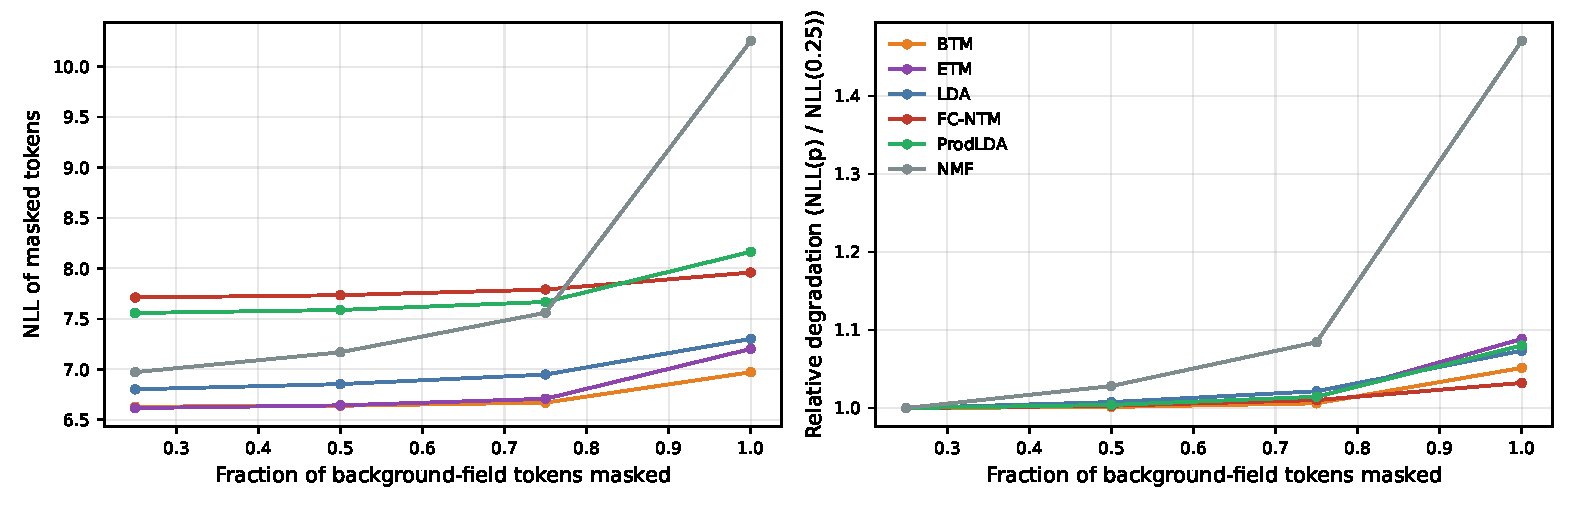
\includegraphics[width=0.86\textwidth]{fig_occlusion_en.pdf}
\caption{Inference behaviour under partial occlusion of the background field (GitHub issues,
seed 11, 2000 test documents). Left: per-token negative log-likelihood of the occluded tokens;
right: relative degradation $\mathrm{NLL}(p)/\mathrm{NLL}(0.25)$, which summarises the relative
increase from the 25\% condition without removing calibration differences. \fcntm{} is trained
with whole-field dropout at $p=0.5$
and has the smallest relative degradation ($\times1.032$); the ratio itself cannot separate
``recovering content from the summary'' from ``being insensitive to the input'', and the absolute
NLL and agreement are not the best, as reported in the text.}
\label{fig:occlusion}
\end{figure}

\subsection{Cross-corpus comparison}

\begin{table}[t]
\centering
\caption{Partial-occlusion behaviour on the three corpora (seeds 11/23/37, mean$\pm$standard deviation; the mask is redrawn per seed). Bold marks the smallest relative degradation per corpus. Field asymmetry is described by the mean background/summary token ratio and by the token-type share of background words that do not occur in the summary of the same document.}
\label{tab:occl-cross}
\small
\setlength{\tabcolsep}{4pt}
\begin{tabular}{@{}llcc@{}}
\toprule
Corpus(Field asymmetry) & Model & Relative degradation & Agreement(100\%) \\
\midrule
\multirow{6}{*}{\shortstack[l]{GitHub issues\\ Length ratio 12.9\\ Background-exclusive 0.877}}
 & \fcntm{} & \textbf{1.029$\pm$0.003} & 0.345 \\
 & LDA & 1.074$\pm$0.000 & 0.424 \\
 & ProdLDA & 1.081$\pm$0.002 & 0.347 \\
 & ETM & 1.088$\pm$0.003 & 0.455 \\
 & BTM & 1.052$\pm$0.001 & 0.438 \\
 & NMF & 1.470$\pm$0.006 & 0.467 \\
\midrule
\multirow{6}{*}{\shortstack[l]{Civil corpus\\ Length ratio 11.2\\ Background-exclusive 0.894}}
 & \fcntm{} & 1.010$\pm$0.001 & 0.673 \\
 & LDA & 1.036$\pm$0.002 & 0.561 \\
 & ProdLDA & 1.027$\pm$0.003 & 0.552 \\
 & ETM & 1.041$\pm$0.001 & 0.655 \\
 & BTM & \textbf{1.007$\pm$0.001} & 0.561 \\
 & NMF & 1.173$\pm$0.001 & 0.655 \\
\midrule
\multirow{6}{*}{\shortstack[l]{AG News\\ Length ratio 3.9\\ Background-exclusive 0.868}}
 & \fcntm{} & 1.018$\pm$0.001 & 0.520 \\
 & LDA & \textbf{1.005$\pm$0.001} & 0.436 \\
 & ProdLDA & 1.026$\pm$0.001 & 0.489 \\
 & ETM & 1.072$\pm$0.001 & 0.554 \\
 & BTM & 1.044$\pm$0.001 & 0.555 \\
 & NMF & 1.408$\pm$0.003 & 0.546 \\
\bottomrule
\end{tabular}
\end{table}

Three conclusions follow. First, the occlusion advantage is measured on only one of the three
corpora and does not follow the length ratio: on GitHub (ratio 12.9) all models degrade measurably
($\times1.028$--$\times1.470$) and \fcntm{} degrades least, beating the best baseline BTM by
$+0.024\pm0.004$ in the ten-seed paired comparison (10/10, $p=0.002$); on the civil corpus, whose
ratio is almost identical (11.2), \fcntm{} (1.010) leaves BTM marginally ahead on the same ratio (1.007 versus 1.010; paired difference $-0.003$, 0/10, $p=0.002$); on AG News (3.9) LDA remains the reference to beat (1.006 versus 1.019).
Second, no training-free statistic agrees with the three corpora: held-out mutual prediction is
slightly higher for GitHub, and the length ratio and background-exclusive share separate GitHub
from AG News but not from the civil corpus. Third, we therefore report these statistics as corpus
descriptions rather than as a pre-training criterion; establishing such a criterion requires
calibration on more corpora and an independent test corpus.

\begin{figure}[t]
\centering
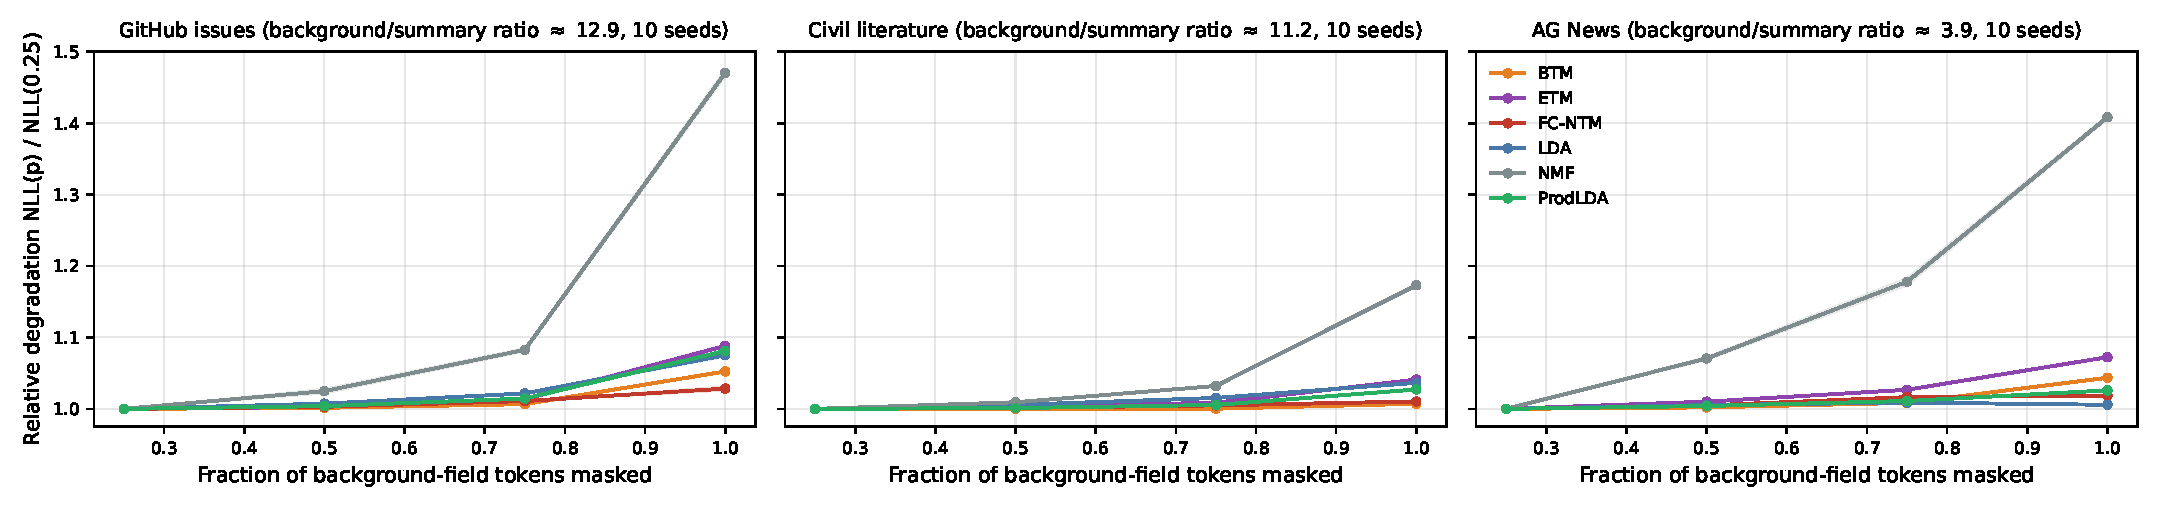
\includegraphics[width=0.86\textwidth]{fig_occlusion_cross_corpus_en.pdf}
\caption{Relative degradation under the same partial-occlusion protocol on three corpora (curves
are means, shading is $\pm1$ standard deviation; \fcntm{}, BTM and LDA cover the ten seeds
11--139, the remaining baselines keep the archived seeds 11/23/37). Left: GitHub issues
(background to summary length ratio $\approx12.9$); middle: civil engineering corpus
($\approx11.2$); right: AG News ($\approx3.9$). Only on GitHub is the degradation of \fcntm{}
clearly below all baselines; on the civil corpus and AG News the smallest degradation belongs to
BTM and LDA respectively, and the gap to \fcntm{} is within 0.003--0.013.}
\label{fig:occl-cross}
\end{figure}

\subsection{Field-restricted read-out}

\begin{table}[t]
\centering
\caption{Field-restricted read-out ($C_V$, mean$\pm$standard deviation over seeds 11/23/37). Every topic--word matrix is truncated to the vocabulary of one field and scored against that field's test text only; ``background view'' is the abstract/body side and ``summary view'' the title side. FC-NTM's summary view is scored on 20--22 scorable topics per seed on GitHub (29--30 on AG News, 26--28 on the civil corpus) because topics whose ten field words never occur in the held-out text get an undefined $C_V$.}
\label{tab:fieldview-baselines}
\small
\setlength{\tabcolsep}{4pt}
\begin{tabular}{@{}llcc@{}}
\toprule
Corpus & Model & Background view $C_V$ & Summary view $C_V$ \\
\midrule
\multirow{5}{*}{GitHub issues}
 & \fcntm{} & 0.697$\pm$0.016 & 0.426$\pm$0.012 \\
 & BTM & \textbf{0.710$\pm$0.011} & 0.396$\pm$0.018 \\
 & NMF & 0.609$\pm$0.004 & 0.433$\pm$0.002 \\
 & LDA & 0.543$\pm$0.011 & 0.466$\pm$0.005 \\
 & ProdLDA & 0.575$\pm$0.006 & \textbf{0.467$\pm$0.034} \\
\midrule
\multirow{5}{*}{AG News}
 & \fcntm{} & 0.566$\pm$0.016 & 0.423$\pm$0.015 \\
 & BTM & \textbf{0.586$\pm$0.015} & 0.399$\pm$0.018 \\
 & NMF & 0.477$\pm$0.015 & 0.444$\pm$0.002 \\
 & LDA & 0.419$\pm$0.007 & \textbf{0.486$\pm$0.006} \\
 & ProdLDA & 0.499$\pm$0.032 & 0.438$\pm$0.007 \\
\midrule
\multirow{5}{*}{Civil corpus}
 & \fcntm{} & \textbf{0.637$\pm$0.015} & 0.408$\pm$0.005 \\
 & BTM & 0.589$\pm$0.014 & 0.382$\pm$0.008 \\
 & NMF & 0.600$\pm$0.009 & 0.398$\pm$0.013 \\
 & LDA & 0.554$\pm$0.008 & 0.415$\pm$0.006 \\
 & ProdLDA & 0.576$\pm$0.025 & \textbf{0.419$\pm$0.012} \\
\bottomrule
\end{tabular}
\end{table}

Field-restricted read-out truncates the topic words to one field's vocabulary and scores them
against that field's own test text. With the shared decoder, the background-view $C_V$ of
\fcntm{} stays close to its full-vocabulary $\beta$ read-out on all three corpora (0.697, 0.566
and 0.637 versus 0.701, 0.586 and 0.633), while the summary view is lower in absolute terms mainly
because a summary contains only 3--5 tokens and the reference corpus is very short, so that column
should be compared within the same protocol only. The cross-model comparison shows that the
read-out is not unique to a two-stream encoder: BTM is slightly better in the background view on
GitHub and AG News (0.710 versus 0.697 and 0.586 versus 0.566), \fcntm{} leads only on the civil
corpus (0.637 versus 0.600 for NMF), and in the summary view LDA and ProdLDA are above \fcntm{}
on all three corpora (0.486 and 0.438 versus 0.423 on AG News). We therefore treat the field view
as a descriptive read-out available to any model with a topic--word matrix, not as evidence of a
unique structural advantage.

\subsection{Ablation: fusion reconstruction and gating}

\begin{table}[t]
\centering
\caption{Three-step fusion ablation on GitHub issues ($K=30$, seeds 11/23/37, same protocol). Within one read-out each row changes exactly one thing: first the fused mixture $\theta_{\mathrm{fuse}}$ is decoded into the reconstruction term (mean fusion), then mean fusion is replaced by a learnable gate (the main model). ``Positive pairs'' counts the seeds whose paired difference against the row above is positive ($C_V$, NPMI).}
\label{tab:fusion}
\small
\begin{tabular}{llcccc}
\toprule
Read-out & Configuration & $C_V$ & NPMI & Positive pairs & UMass \\
\midrule
\multirow{3}{*}{$\beta$} & No fusion & 0.721$\pm$0.016 & 0.266$\pm$0.012 & --- & $-$2.63 \\
 & Mean fusion + fusion recon. & 0.708$\pm$0.016 & 0.245$\pm$0.013 & 1/3, 0/3 & $-$2.98 \\
 & Gated fusion (main model) & 0.701$\pm$0.016 & 0.233$\pm$0.012 & 0/3, 0/3 & $-$3.16 \\
\midrule
\multirow{3}{*}{cTFIDF} & No fusion & 0.714$\pm$0.001 & 0.262$\pm$0.007 & --- & $-$1.86 \\
 & Mean fusion + fusion recon. & 0.728$\pm$0.007 & 0.275$\pm$0.015 & 3/3, 3/3 & $-$1.91 \\
 & Gated fusion (main model) & 0.727$\pm$0.022 & 0.274$\pm$0.026 & 1/3, 1/3 & $-$1.90 \\
\bottomrule
\end{tabular}
\end{table}

The three-step ablation separates two questions: whether the fused mixture receives its own
reconstruction term, and whether fusion is averaged or gated. The fusion-reconstruction term is
effective, but only for the read-out that uses the fused posterior: adding it under mean fusion
raises the class TF--IDF $C_V$ and NPMI by 0.014 and 0.013 (3/3 seeds) while lowering the $\beta$
read-out by 0.013 and 0.021. Replacing mean fusion by a gate brings no further gain in this corpus
and protocol (class TF--IDF differences $-0.001$ and $-0.000$, 1/3 seeds; $\beta$ read-out
$-0.007$ and $-0.012$, 0/3). This conclusion has a precise boundary: without the fusion
reconstruction term the gate receives no gradient and the model degenerates exactly to mean fusion,
so the experiment cannot separate the value of the gate parameters from the value of the fusion
objective; we report the absence of an observed gain rather than claiming that a trained gate is
useless in general.

\subsection{Ablation: core components}

\begin{table}[t]
\centering
\caption{Core-component ablation on three corpora and two read-outs ($K=30$, seeds 11/23/37, 700-epoch budget, all other settings identical to the main model). Each column switches off one component: cross-field reconstruction of both streams, the JS consistency weight, field-level word masking, and whole-field dropout; the fusion-reconstruction term is kept in all columns. Values are mean paired $\Delta C_V$ (negative means the component matters), parentheses count positive pairs.}
\label{tab:core-ablation}
\small
\setlength{\tabcolsep}{5pt}
\begin{tabular}{llcccc}
\toprule
Corpus & Read-out & $-$Cross-field recon. & $-$JS consistency & $-$Word masking & $-$Field dropout \\
\midrule
GitHub & $\beta$ & $+$0.021 (2/3) & $-$0.001 (1/3) & $-$0.012 (1/3) & $-$0.023 (1/3) \\
GitHub & Class TF-IDF & $-$0.005 (1/3) & $+$0.004 (2/3) & $-$0.004 (1/3) & $-$0.021 (1/3) \\
\midrule
AG News & $\beta$ & $-$0.011 (2/3) & $+$0.003 (1/3) & $-$0.026 (0/3) & $-$0.010 (1/3) \\
AG News & Class TF-IDF & $-$0.022 (0/3) & $-$0.002 (1/3) & $-$0.043 (0/3) & $-$0.023 (1/3) \\
\midrule
Civil corpus & $\beta$ & $-$0.022 (0/3) & $+$0.001 (2/3) & $-$0.010 (1/3) & $+$0.001 (1/3) \\
Civil corpus & Class TF-IDF & $-$0.019 (0/3) & $-$0.002 (0/3) & $-$0.012 (0/3) & $-$0.034 (0/3) \\
\bottomrule
\end{tabular}
\end{table}

Four components are switched off one at a time. First, removing the JS consistency term causes no
consistent change in topic quality on any corpus or read-out (all six cells
$|\Delta C_V|\leq0.004$, none with a clear positive paired majority): in this
parameterisation the fused representation is trained by the fusion-reconstruction objective, not by
pulling the two posteriors together. Second, the observed effect of cross-field reconstruction
and word masking depends on the corpus: on GitHub, removing cross-field reconstruction even raises
the $\beta$ read-out by 0.021 (2/3 seeds) and costs only 0.005 in the class TF--IDF read-out, while
on AG News and the civil corpus both read-outs drop when either component is removed (cross-field
reconstruction $-0.011/-0.022$ and $-0.022/-0.019$; word masking $-0.026/-0.043$ and
$-0.010/-0.012$, with all class TF--IDF columns at 0/3). Third, whole-field dropout acts mostly on
the class TF--IDF read-out and is consistently beneficial on two of the three corpora only: it
lowers both read-outs on GitHub
and AG News but changes the $\beta$ read-out of the civil corpus by only $+0.001$ while lowering
its class TF--IDF read-out by 0.034. Fourth, field asymmetry does not explain the component-level
differences: the civil corpus has almost the same length ratio as GitHub (11.2 versus 12.9) yet
behaves like AG News (3.9). The scope of the ablation is also limited: it switches off the
per-stream cross-field reconstruction while the fused reconstruction term still rebuilds both
fields, so it does not cut all information flow between fields.

\subsection{Sensitivity to the fusion weight}

\begin{table}[t]
\centering
\caption{Sensitivity to the fusion-reconstruction weight $\lambda_f$ on GitHub issues (gated fusion, seeds 11/23/37). $\lambda_f=0$ is the no-fusion setting, $\lambda_f=0.5$ is the value used throughout; all other settings match the main model.}
\label{tab:weight}
\small
\setlength{\tabcolsep}{4pt}
\begin{tabular}{lcccc}
\toprule
\multirow{2}{*}{$\lambda_f$} & \multicolumn{2}{c}{$\beta$ read-out} & \multicolumn{2}{c}{Class TF--IDF} \\
 & $C_V$ & NPMI & $C_V$ & NPMI \\
\midrule
0 & 0.721$\pm$0.016 & 0.266$\pm$0.012 & 0.714$\pm$0.001 & 0.262$\pm$0.007 \\
0.25 & 0.697$\pm$0.015 & 0.217$\pm$0.031 & 0.713$\pm$0.015 & 0.262$\pm$0.004 \\
0.5 & 0.701$\pm$0.016 & 0.233$\pm$0.012 & 0.727$\pm$0.022 & 0.274$\pm$0.026 \\
1.0 & 0.716$\pm$0.012 & 0.246$\pm$0.026 & 0.723$\pm$0.012 & 0.277$\pm$0.018 \\
\bottomrule
\end{tabular}
\end{table}

At $\lambda_f=0.25$ the class TF--IDF read-out is essentially the no-fusion result ($C_V$ 0.713
versus 0.714) while the $\beta$ read-out has already dropped by 0.024; between 0.5 and 1.0 the
class TF--IDF gain is stable (0.727 versus 0.723, NPMI 0.274 versus 0.277, differences below
0.005), and the $\beta$ penalty narrows from $-0.020$ to $-0.005$ relative to $\lambda_f=0$.
The value 0.5 used throughout is therefore a conservative compromise.

\subsection{Whole-field occlusion}

\begin{table}[t]
\centering
\caption{Whole-field occlusion at inference time ($K=30$, final configuration, 700-epoch budget). $\Delta C_V$ is the coherence difference between full-field and occluded inference under the same read-out; $\Delta\mathrm{NLL}$ is the per-token increase; agreement is the fraction of documents whose most probable topic is unchanged. The two rows of a corpus use the same seeds, isolating the effect of the training-time dropout setting.}
\label{tab:occlusion}
\small
\setlength{\tabcolsep}{4pt}
\begin{tabular}{llcccccc}
\toprule
Corpus & Training setting & $C_V^{\mathrm{full}}$ & $C_V^{\mathrm{occ}}$ & $\Delta C_V$
 & $\Delta\mathrm{NLL}$(per token) & Agreement & Mean JS \\
\midrule
GitHub & Dropout ($p=0.5$) & 0.727 & 0.717 & $+$0.009 & $+$0.241 & 0.345 & 0.082 \\
       & No dropout & 0.705 & 0.725 & $-$0.020 & $+$0.242 & 0.346 & 0.092 \\
\midrule
Civil corpus & Dropout ($p=0.5$) & 0.636 & 0.627 & $+$0.009 & $+$0.103 & 0.673 & 0.033 \\
        & No dropout & 0.602 & 0.597 & $+$0.005 & $+$0.125 & 0.642 & 0.039 \\
\midrule
AG News & Dropout ($p=0.5$) & 0.612 & 0.594 & $+$0.018 & $+$0.232 & 0.520 & 0.049 \\
        & No dropout & 0.589 & 0.582 & $+$0.007 & $+$0.269 & 0.498 & 0.060 \\
\bottomrule
\end{tabular}
\end{table}

Deleting the background field entirely leaves topic-word coherence almost unchanged (all six cells
within $\pm0.02$, with sign flips across seeds on GitHub), so coherence is insensitive to field
loss and the information loss must be read from the document-level posterior and the word-level
prediction: about 66\% (GitHub) and 48\% (AG News) of the documents change their most probable
topic, and the per-token NLL rises by 0.24/0.23 with dropout training (0.24/0.27 without).
Training with whole-field dropout changes the shape of the posterior rather than the calibration of
word prediction: it lowers the per-token increase from 0.269 to 0.232 and the posterior JS from
0.060 to 0.049 on AG News, is directionally the same on the civil corpus
(0.125$\to$0.103, JS 0.039$\to$0.033), and shows no increase difference on GitHub
(0.242 versus 0.241) where only the JS slightly improves. Two corpora therefore show reduced
posterior drift under field loss, which cannot replace absolute prediction accuracy.

\subsection{Concatenated-field single-encoder control}

To compare the full method with a single-encoder alternative under the same budget we train a
control on the concatenated bag of words $[x_{\mathrm{bg}};x_{\mathrm{sm}}]$ with the same shared
linear decoder, field weights, KL warm-up and orthogonality penalty; whole-field dropout is
emulated by zeroing the background half of the input, and there is no fusion or consistency
term. The concatenated input doubles the first encoder layer, keeping the parameter count
comparable (a 1.5\% difference), and both models use the same budget, vocabulary and read-outs
on all three corpora (seeds 11/23/37).

\begin{table}[t]
\centering
\caption{Concatenated-field single-encoder control (seeds 11/23/37; same budget, vocabulary and read-outs). $\Delta$ is \fcntm{} minus the control, with positive pairs in parentheses.}
\label{tab:concat}
\small
\begin{tabular}{llcccc}
\toprule
Corpus & Read-out & \fcntm{} & Concatenated & $\Delta$ (positive pairs) \\
\midrule
GitHub & $\beta$ & 0.701$\pm$0.016 & 0.683$\pm$0.014 & $+$0.017 (2/3) \\
GitHub & Class TF--IDF & 0.727$\pm$0.022 & 0.710$\pm$0.020 & $+$0.017 (1/3) \\
AG News & $\beta$ & 0.586$\pm$0.026 & 0.574$\pm$0.019 & $+$0.012 (2/3) \\
AG News & Class TF--IDF & 0.612$\pm$0.014 & 0.584$\pm$0.009 & $+$0.028 (3/3) \\
Civil corpus & $\beta$ & 0.633$\pm$0.014 & 0.623$\pm$0.014 & $+$0.010 (2/3) \\
Civil corpus & Class TF--IDF & 0.636$\pm$0.014 & 0.606$\pm$0.014 & $+$0.029 (2/3) \\
\bottomrule
\end{tabular}
\end{table}

The control is competitive everywhere, so the two-stream structure is not a necessary condition
for topic quality. After the validation-mode correction the mean difference favours \fcntm{} in
every corpus--read-out cell ($+0.010$ to $+0.029$ $C_V$), but the paired majorities are mixed
(1/3 to 3/3) and the gaps remain at the scale of the seed-to-seed variation with three seeds per
cell, so the two-stream architecture is reported as a matched design choice rather than a source of unconditional coherence gains.
The control also supports
field-restricted read-out and title-only inference, so those read-outs are not exclusive to the
two-stream design either.

\subsection{Title-only routing on the civil corpus}

When the abstract of a record is missing, can its title still be routed to an interpretable civil
subfield? The evaluation labels are the OpenAlex primary topics of each record --- external
automatic labels from a classifier rather than expert ground truth; the frozen snapshot (topic
IDs, fetch date) is released with the code, and the label set is the 15 most frequent topics of
the training split, covering 42.9\% of the test records (2000-record test split). Every model
infers a topic distribution from the title only (\fcntm{} and the control use their
missing-background inference path); the per-model topic-to-label mapping is a supervised step ---
the majority training label of each argmax topic, with the training-label prior as fallback for
topics that take no training record (three test records in one run triggered this fallback) ---
fitted on the same title-only inference, so the pipeline is an unsupervised representation with
a supervised training-split mapping. Accuracy and
macro-F1 are reported per seed; a supervised TF--IDF logistic regression on the same titles
serves as a reference point, and \fcntm{} with the full fields as an upper reference.

\begin{table}[t]
\centering
\caption{Title-only routing to the 15 most frequent OpenAlex topics of the civil corpus (seeds 11/23/37; 857 test records, coverage 42.9\%). The TF--IDF classifier is supervised and serves as a reference point, not as a topic model.}
\label{tab:archival}
\small
\begin{tabular}{llcc}
\toprule
Method & Input & Accuracy & Macro-F1 \\
\midrule
TF--IDF logistic regression (supervised) & title & 0.810 & 0.805 \\
\fcntm{} & title + abstract & 0.719$\pm$0.016 & 0.676$\pm$0.032 \\
\fcntm{} & title only & 0.664$\pm$0.004 & 0.624$\pm$0.013 \\
Concatenated control & title only & 0.653$\pm$0.012 & 0.614$\pm$0.034 \\
BTM & title only & 0.600$\pm$0.013 & 0.529$\pm$0.043 \\
LDA & title only & 0.532$\pm$0.039 & 0.458$\pm$0.057 \\
\bottomrule
\end{tabular}
\end{table}

Topic-based routing from titles alone recovers a substantial part of the full-field signal
(0.664 versus 0.719 accuracy) and clearly outperforms the classical topic-model baselines
(LDA 0.532, BTM 0.600), but it remains well below a supervised TF--IDF classifier trained on the
same titles (0.810); the topic representation is learned without labels, while the topic-to-label
mapping uses training labels, which is why the supervised classifier retains its advantage. The
concatenated control reaches 0.653 against 0.664 for \fcntm{}, but the three paired per-seed
differences are not consistent in direction and the gap is small relative to the per-seed
variation, so the two architectures operate within comparable ranges on this task. The task
is a routing aid under a fixed label set, not a substitute for supervised classification, and
its accuracy depends on the 42.9\% label coverage of the 15-topic set.

\section{Discussion and Limitations}

The value of dual-field topic modelling has to be stated in parts. What is reproducible is the
behaviour at the \emph{representation} level: one trained model yields field-restricted topic words,
and it still infers topic proportions when the background field is missing (on GitHub about 66\% of
the documents change their most probable topic and the per-token NLL rises by 0.24). What is
corpus-dependent is the advantage on \emph{generic} coherence metrics: under the matched read-out,
the ten-seed comparison supports \fcntm{}-cTFIDF being $+0.028$ $C_V$ above BTM on GitHub
(95\% CI excludes zero, 9/10 seeds) and $+0.049$ on the civil corpus (10/10) but $-0.009$ on
AG News (3/10); on the civil corpus the native $\beta$ read-out is also above BTM ($+0.061$,
10/10). This differs from the simple
hypothesis that complementary corpora benefit and redundant ones suffer, for two reasons: coherence
metrics are sensitive to implementation details such as the decoding path, the training budget and
Monte-Carlo noise, so measuring under one protocol is more reliable than extrapolating from
intuition; and the held-out redundancy measures show that GitHub is in fact slightly the more
predictable of the two corpora. Redundancy is therefore reported as a description of the field
relation, not as a predictor of the direction of the gain.

For engineering document management the protocol has direct uses: the field-restricted read-out
matches the way titles and abstracts are actually written, the occlusion diagnostic corresponds
to estimating topics when abstracts are missing, and the title-only routing experiment shows that
such topics can be mapped to civil subfields with moderate accuracy against independent OpenAlex
labels. Even though the generic coherence gain over the concatenated control is limited, these
read-outs are usable engineering outputs.

The limitations are as follows. First, all three corpora are English and the field split follows
existing title/body structure; automatic field-boundary detection is untested, and the GitHub
background field has a long tail (up to 20532 tokens) that the sentence-embedding baselines truncate
at 128 tokens, for which the Supplementary Material reports a window-pooling control. Second, the
redundancy measures are computed on two corpora with almost the same held-out predictability
($\rho^2_{\mathrm{cca}}$ 0.306 versus 0.245) while the ten-seed gain appears on one of them, so the two corpora define the current calibration range, and a redundancy-based pre-training criterion will need calibration on additional corpora and an independent test set. Third, the non-parametric
baselines choose their own topic numbers (Top2Vec degrades to 2--4 topics on AG News) and are shown
for reference only. Fourth, field-restricted read-out is available to any model with a
topic--word matrix and is not unique to a two-stream encoder. Fifth, the masking rate, the
whole-field dropout probability and the fusion weight are empirical values whose interaction with
corpus size and field ratio is not characterised; the in-house variational baselines and \fcntm{}
use 20\% of the training documents for early stopping (the official CombinedTM keeps its own
held-out split), while the class TF--IDF read-out of \fcntm{} aggregates the full training set, so
the number of documents used for optimisation and for read-out differs. Sixth, all
numbers come from one protocol ($K=30$, 700-epoch budget, unified read-out and evaluation
vocabulary): \fcntm{} and BTM are extended to ten seeds on all three corpora (and LDA's occlusion
curves for the new seeds), while the remaining baselines and the main tables stay at three seeds.
Seventh, the concatenated-field control and the title-only routing task are run for three seeds
per cell and against one label source (OpenAlex primary topics), so their differences should be
read at the scale of the seed-to-seed variation. Finally, no independent confirmation corpus is
used.

\section{Summary and Conclusions}

This paper presented \fcntm{}, a field-cooperative neural topic model for dual-field short texts:
two conditional variational streams share one linear topic decoder, cross-field reconstruction and a
consistency regulariser encode the field relation into a shared topic space, and field-level word
masking and whole-field dropout handle partial and complete field absence. A single trained model
supports a decoder $\beta$ read-out and a class TF--IDF read-out under one evaluation vocabulary,
which removes the vocabulary and topic-length confounds of cross-model comparison.

On civil engineering title--abstract records and two public corpora the results depend on the
corpus. Under the read-out-matched protocol the ten-seed comparison gives $+0.028$ $C_V$ over BTM on
GitHub (95\% CI $[+0.012,+0.043]$, 9/10) and $-0.009$ on AG News (CI includes zero, 3/10); on the
civil corpus both read-outs favour \fcntm{} by a larger margin ($+0.049$ class TF--IDF and
$+0.061$ $\beta$, 10/10), and on the two public corpora BTM keeps its lead under the native $\beta$ read-out. A same-budget concatenated-field single encoder is close on every corpus (mean
$\Delta C_V$ $+0.010$--$+0.029$ with mixed paired majorities), and title-only routing reaches
0.66 accuracy against independent OpenAlex labels (42.9\% coverage). Two field-relation measures were tested and
neither predicts the gain: the corpora have similar redundancy, and occluding the background field
leaves coherence almost unchanged while changing the document-level posterior and the word-level
prediction. The contribution of this paper is therefore scoped: \fcntm{} provides reproducible
field-restricted read-outs and missing-field inference behaviour, and read-out-matched advantages
supported by ten seeds on the civil corpus and on GitHub. The complete \fcntm{} configuration shows
small mean coherence gains over the concatenated control, which is reported as a matched configuration-level comparison. Whether field structure
is worth the extra modelling cost should be measured on the target corpus with the protocol used
here rather than decided from redundancy beforehand.

\section{Data Availability Statement}

All data, models, and code that support the findings of this study are available from the
corresponding author upon reasonable request; the archived corpus splits, model checkpoints and
per-seed results accompany this submission.

\section{Supplemental Materials}

The supplementary material contains the auxiliary experiments and controls, the data and metric
notes, and the case-study tables cited in the text.

% bibliography style is set by ascelike-new.cls
\bibliography{main_asce}

\end{document}
